\documentclass{book}
\usepackage{graphicx} % Required for inserting images

\usepackage[utf8]{inputenc}
\usepackage[T1]{fontenc}
\usepackage{listings}
\usepackage{appendix}
\usepackage{siunitx}
\usepackage{multirow}
\usepackage{mhchem}
\usepackage{natbib}
\usepackage{astrojournals}
\bibliographystyle{aasjournal}
\renewcommand{\lstlistingname}{Algoritmus}

\title{Avances de tesis}
\author{r.reyes }
\date{December 2023}

\begin{document}

\maketitle

\tableofcontents

\newpage

\chapter{Introducción}

Los \text{glóbulos} son grandes concentraciones de gas y polvo en el medio interestelar que se cree que se forman por inestabilidades térmicas, colapso gravitacional o o turbulencia. Estos glóbulos se pueden formar en regiones de formación estelar masiva o en nebulosas alrededor de estrellas evolucionadas y en realidad tienen muchos tamaños de escala.

Cuando nos referimos a los glóbulos en regiones de formación estelar masiva, estos tienden a ser de un gran tamaño comúnmente, $\sim$\SI{0.1}{pc}, e interactúan con la radicación UV (ultravioleta) de las estrellas jóvenes masivas como estrellas tipo O, mientras que en nebulosas alrededor de estrellas evolucionadas son de un tamaño más pequeño, $\sim$\SI{e-2}{pc}. En algunos casos dependiendo que tan intensa es la radiación incidente por parte de la o las estrellas, podemos ver un \textit{flujo fotoevaporativo} por parte del glóbulo, el cual es causado por la radiación incidente.

Los primeros glóbulos fueron observados por Bart Bok en 1940, estos glóbulos son nubes oscuras, relativamente pequeños comparados con otras regiones de formación estelar, que tienen gran cantidad de gas y polvo. Estos glóbulos contienen principalmente hidrógeno molecular en su interior, así como también pueden tener otras moléculas, metales e incluso algunos silicatos. Si bien puede tener formación estelar en su interior no podemos ver la radiación de las estrellas ya que es absorbida por el hidrógeno atómico y el polvo, es por eso que se ven oscuras. Sin embargo, estos pueden ser radiados externamente, en regiones de formación estelar, por estrellas jóvenes masivas que se están formando cerca, y en algunos casos podemos ver el frente de ionización.

\begin{figure}[h!]
    \centering
    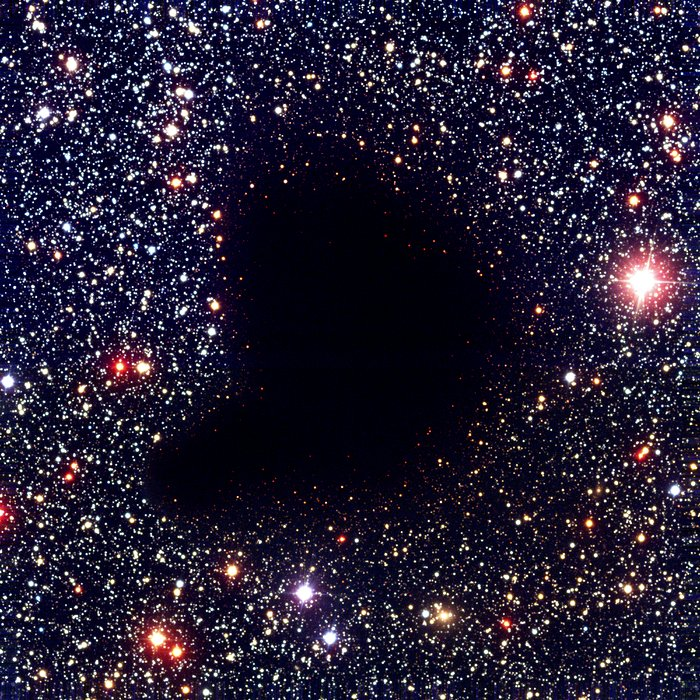
\includegraphics[width=0.75\textwidth]{images Chapter 1/C1_Bok_globule.jpg}
    \caption{Imagen de Banard 68, un ejemplo de un glóbulo de Bok, visto con Very Large Telescope FORS1 en 440 nm, 557 nm y 768 nm. Se puede apreciar una zona oscura y lo que pareciera ser enrojecimiento de las estrellas por polvo en la superficie del glóbulo. En esta imagen podemos ver que no hay evidencia de alguna fotoevaporación externa por parte de estrellas. \citep{Alves:2001}.}
    \label{fig:Banard}
\end{figure}

Esta interacción entre estrellas y glóbulos se puede dar a diferentes escalas, lo que nos da una gran variedad de estructuras. Entre las de mayor tamaño se encuentran lo que parecen ser columnas, pilares o trompas de elefantes, como se les conoce en la literatura, que llegan a tener un tamaño de $\sim$\SI{1}{pc} y una densidad del orden de \SI{e3}{cm^{-3}}. En algunas ocasiones tienden a llamar glóbulo en la literatura a los que, al igual que lo anterior a mencionado, tienen una gran estructura también pero son más densos, $\sim$ \SI{e4}{cm^{-3}}. Esta interacciones también se puede dar dentro de regiones HII, como vemos en la figura \ref{fig:Pillars}.

\begin{figure}[h]
    \centering
    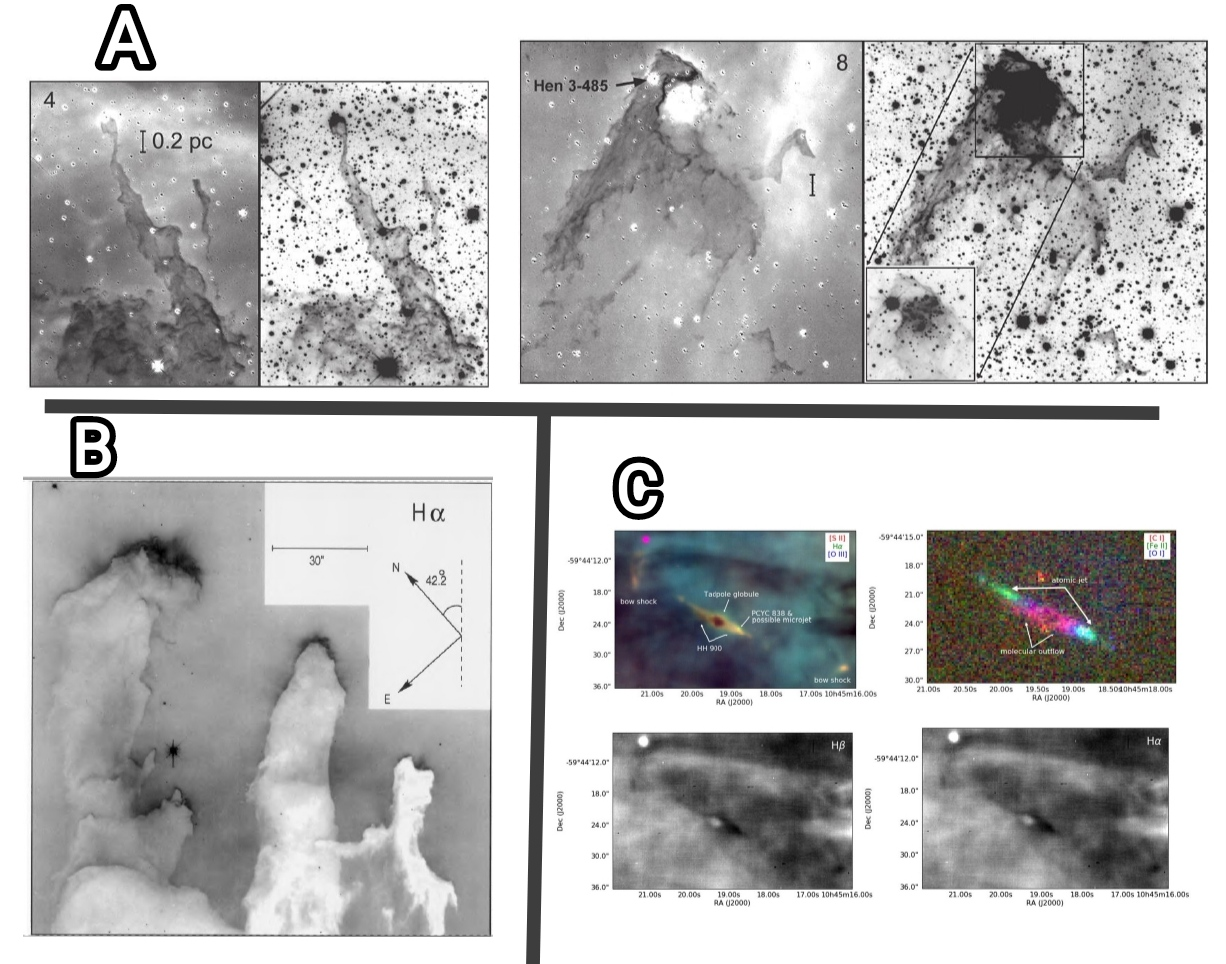
\includegraphics[width=1 \textwidth]{images Chapter 1/C1_Pillars.jpg}
    \caption{En \textbf{A} vemos dos ejemplos de pilares, donde la imagen derecha de cada ejemplo es vista a 2.12$\mu$m (\SI{}{H_2}), y la imagen izquierda es \SI{}{H_2-Br_{\gamma}} \citep{Hartigan:2015}. \textbf{B}, ejemplo de una trompa de elefante, es una imagen de M16 tomada con WFPC2 con e filtro F656N, los \SI{30}{\arcsecond} corresponden \SI{9e17}{cm} (\SI{0.29}{pc}) \citep{JJHester:1996}. \textbf{C} es el outflow de Tadpole globule, el cual consta del sistema HH900 jet+outflow, la imagen de abajo es vista en \SI{}{H_\alpha} con el continuo 
    \citep{MeganReiter:2019}. }
    \label{fig:Pillars}
\end{figure}

En escalas más pequeñas están lo que se conoce como EGGs (Evaporating Gaseous Globule), en escalas de $\sim$\SI{0.1}{pc}, y los proplyds, en escalas de $\sim$\SI{e-2}{pc}. 

No solo se da en regiones de formación estelar, como ya hemos dicho, también hay dentro de nebulosas alrededor de estrellas evolucionadas donde se les conoce más comúnmente como \textit{nudos}, un ejemplo de esto es la imagen \textbf{D} de la figura \ref{fig:nudos}. Estos nudos son los que estudiaremos más fondo en este trabajo.

\begin{figure}[h]
    \centering
    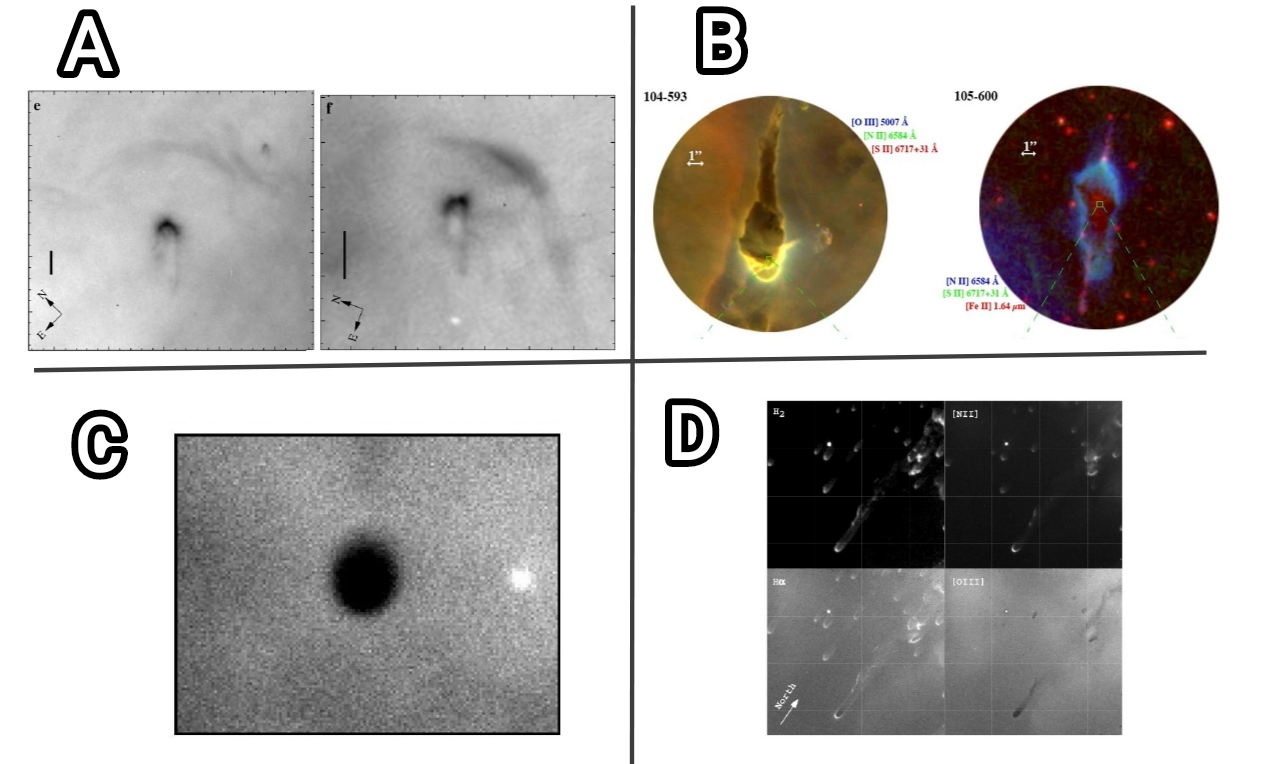
\includegraphics[width=1 \textwidth]{images Chapter 1/C1_Globulettes.jpg}
    \caption{En \textbf{A} vemos proplyds con su bowshock en Orion tomado con HST planetary camera, la barra negra indica una medida de \SI{1}{\arcsecond} que corresponde a 430 AU (\SI{2e-3}{pc}) \citep{Garcia-Arredondo:2001}. \textbf{B} son ejemplos de EGGs en Carina, tomado con WFC3, ACS, WFPC2 \citep{Mesa-Delgado:2016}. \textbf{C} es el globulette denso RN88 visto en \SI{}{H_\alpha} con un diámetro de \SI{6}{\arcsecond} (\SI{4e-2}{pc}) en la nebulosa de Rosette \citep{GFGahm:2013}. \textbf{D} son ejemplos de nudos en la nebulosa de la Hélice, los mosaicos tienen una medida de \SI{47.5}{\arcsecond}$\times$\SI{44.8}{\arcsecond} (\SI{4.76e-2}{pc}$\times$\SI{4.49e-2}{pc}) \citep{O'Dell:2007}. }
    \label{fig:nudos}
\end{figure}



\section{Flujos de foto evaporación ionizada}

Todos los ejemplos de las figuras \ref{fig:Banard}, \ref{fig:Pillars} y \ref{fig:nudos} se encuentran ya sea en regiones de formación estelar o en nebulosas alrededor de estrellas evolucionadas. 

Lo interesante en todos estos ejemplos es la forma que toman al interaccionar con las estrellas más masivas que se encuentran cerca, esto para los glóbulos que se encuentran en regiones de formación estelar.  Mientras que los que se encuentran en nebulosas planetarias, interactúan con la estrella evolucionada. Durante estas interacciones en algunos casos podemos ver lo que se conoce como flujos fotoevaporativos, los cuales explicaremos mejor a continuación.

Para que se pueda dar esta interacción y crear un flujo fotoevaporativo por parte de la nube es necesario que la estrella ionizante sea masiva o tenga un gran flujo ionizante como para poder ionizar el gas neutro. \cite{OortySpitzer_1955} explican a manera detallada como es la interacción entre una estrella tipo O y una nube interestelar de gas neutro. Con esto podemos explicar de una mejor manera como es la interacción en regiones de formación estelar masiva. Recordemos que en las regiones de formación estelar hay michas estrellas nuevas que emiten principalmente en radio o infrarrojo, por lo que no todas las estrellas nuevas pueden ionizar el gas neutro.

\cite{OortySpitzer_1955} consideran tres partes importantes para esto, la estrella ionizante, la nube interestelar de gas neutro y la región que hay entre la estrella y la nube interestelar. La nube interestelar debe ser mucho más densa y fría que la región que hay entre la estrella y la nube como vemos en la figura \ref{kahn_zones}.

\begin{figure}[h]
    \centering
    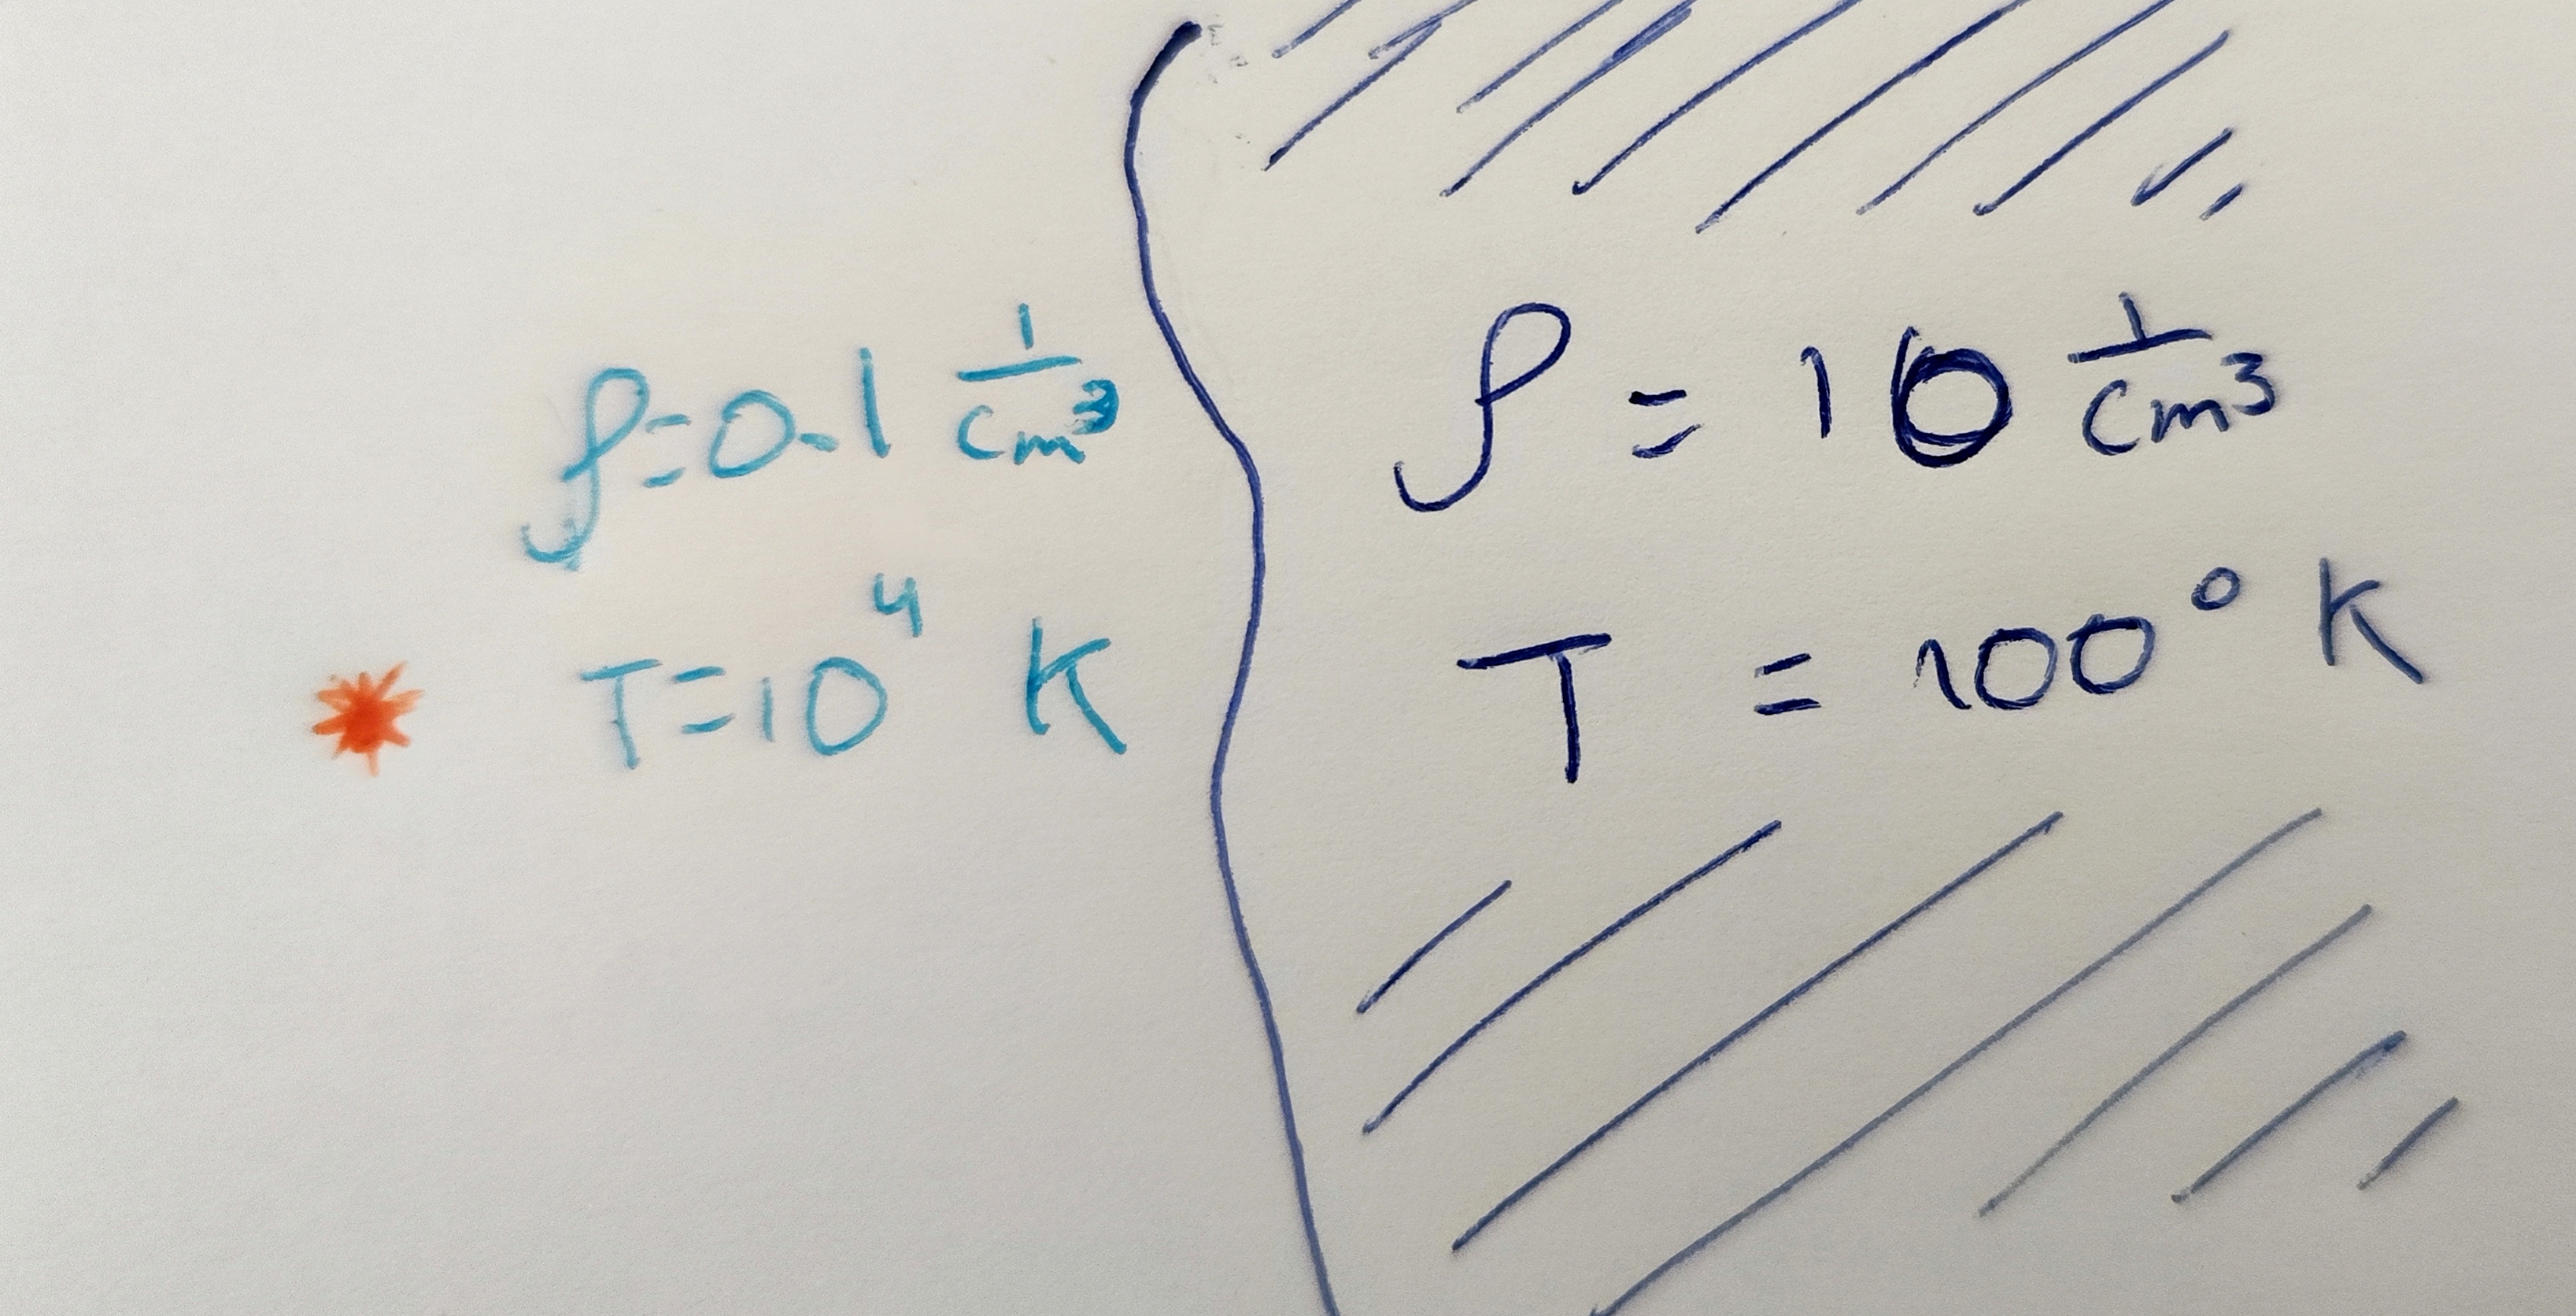
\includegraphics[width=0.5 \textwidth]{images Chapter 1/C1_Kahn.jpg}
    \caption{Esquema inicial utilizado en \cite{Kahn:1954}}
    \label{kahn_zones}
\end{figure}

Cuando la radiación UV comienza a calentar el gas de la nube, el gas ionizado comienza a expandirse en dirección a la estrella, esto ya que en esta dirección la densidad es menor que la de la nube y puede expandirse libremente. De esta manera mientras el gas ionizado va en dirección a la estrella, el frente de ionización se va alejando. A este efecto se le conoce como efecto rocket.

En un inicio esta radiación ioniza el gas a una tasa muy rápida causando una ``tormenta de partículas ionizantes'' que viene por parte de la nube, conforme esto va evolucionando se crea una capa aislante alrededor de la nube. Mientras esto ocurre hay un choque interno que va viajando a través de la nube a la parte trasera. Para que esto ocurra \cite{Kahn:1954} da cierto criterios, en los cuales dice que la radiación no debe ser muy débil o demasiado fuerte.

\section{Estrellas Wolf-Rayet y sus vientos}

Las estrellas Wolf-Rayet (WR) son estrellas evolucionadas de estrellas masivas, como estrellas tipo O, y fueron nombradas así después de que Charles Wolf y Georges Rayet identificaran 3 estrellas en Cygnus con sus  anchas líneas de emisión que las caracterizan muy bien. 

Estas estrellas se caracterizan por el cociente que hay entre sus líneas de emisión intensa que las caracterizan. \cite{Smith:1968} las clasifica principalmente como WN a aquellas que son abundantes en He y N, WC a las que son abundantes en He y C. Además les pone un número para identificar esencialmente si son tipo tardío o temprano.

\begin{table}[h!]
    \begin{center}
        \begin{tabular}{|c|c|}
        \hline
        \multicolumn{2}{|c|}{Clasificación de estrellas WR} \\ \hline
        Clasificación    & Tipo de estrellas\\ \hline
        WN2--5     & Tipo temprana, WNE (Early WN)\\
        WN7--9 & Tipo tardía, WNL (Late WN) \\
        WC4--6 & WCE\\
        WC7--9 & WCL \\ \hline
        \end{tabular}
    \caption{Principal clasificación de estrellas WR  según sus líneas de emisión. Dentro de las WC, las que se clasifican como WC6 pueden ser de tipo tardía o temprana.}
    \label{tab:WR-clasificacion}
    \end{center}
\end{table}

También están las estrellas WO que son abundantes en He y O, pero en realidad son una extensión de las WCE. Para las estrellas que son ricas en H se les pone también una ``h'' \citep{SSM:1996}.

Estas estrellas se caracterizan principalmente por sus fuertes vientos que pueden ser del orden de $\sim$\SI{1000}{km/s}, los cuales provocan sus líneas de emisión anchas. Así como también tienen una alta pérdida de masa $\sim$2--\SI{10e-5}{M_\odot/yr}. Típicamente son estrellas de 10--25\SI{.}{M_\odot} que son descendientes de estrellas tipo O y se caracterizan por tener intensas líneas de emisión de libre-libre desde el $\mu$m hasta el cm \citep{crowther:2007}.

\section{Nebulosa M1-67}

M1-67 es la nebulosa alrededor de la estrella WR-124, que tiene índice espectral WN8h. En la figura \ref{} vemos que la imagen tomada con el telescopio espacial Hubble (HST) en H$\alpha$ se puede notar una gran presencia de H en toda la nebulosa, mientras que en la imagen tomada por el telescopio espacia James Webb (JWST), tomada en varios filtros de los cuales incluye en  el infrarrojo cercano, podemos ver una gran estructura. Algo muy notorio a simple vista en la imagen de JWST es que podemos apreciar la presencia de algunos nudos en la nebulosa como se ve  en la figura \ref{fig:zones}.

\begin{table}[h]
    \centering
    \begin{tabular}{|c|c|}
        \hline
        \multicolumn{2}{|c|}{Parámetros de la estrella WR 124} \\ \hline
         D & \SI{5.429}{kpc} \\
         $v_\infty$ & \SI{710}{km/s} \\
         $\dot{M}$ & \SI{2e-5}{M_\odot/yr} \\
         L & \SI{1.25e49}{s^{-1}} \\
         $F_{H_\alpha}$ & \SI{3e-14}{erg cm^{-2} s^{-1}} \\ \hline
    \end{tabular}
    \caption{Parámetros de WR 124}
    \label{tab:parametros WR-124}
\end{table}

\begin{figure}[h]
    \centering
    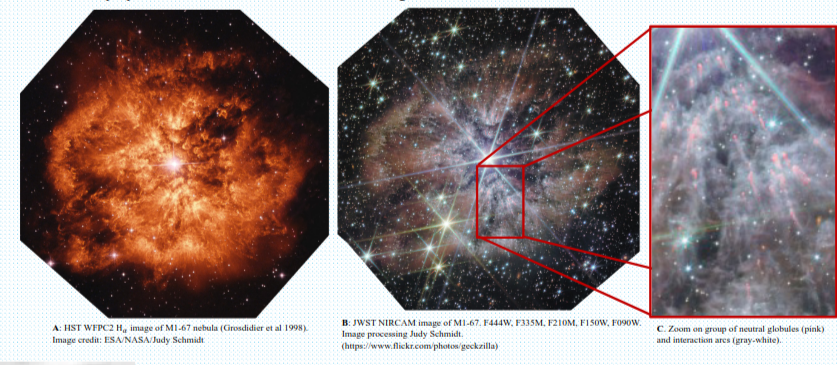
\includegraphics[width=0.75\textwidth]{images Chapter 1/C1_WR124.png}
    \caption{...}
    \label{fig:zones}
\end{figure}

Podemos ver como muchos detalles en cada uno de los filtros, en especial de como podemos ver en color rosa lo que parece ser choques de una gran acumulación de gas neutro que está interactuando con el viento de la estrella, y al rededor de ellos vemos una morfología similar a la de los proplyds que hay en otras nubes moleculares. También podemos ver como estos tienen una estela en la parte más lejana de la interacción, pero para nuestro estudio solo nos concentraremos solo en la parte más central.

\chapter{Modelos analíticos de flujos foto evaporativos interactuando con una presión externa}

En este capitulo vamos  a describir nuestro modelo, esto con el fin de explicar la interacción que hay entre el flujo foto evaporativo de unos glóbulos, que es provocado por la radiación de una estrella, y el viento estelar, que proviene de la misma estrella. Tomaremos estos glóbulos separados unos de otros, por lo que comenzaremos por describir la interacción del flujo foto evaporativo de un solo glóbulo y el viento estelar.

Para nuestro modelo estamos considerando que los glóbulos contienen principalmente hidrógeno neutro y tienen una forma esférica. Estos glóbulos deben estar lo suficientemente cerca de una estrella masiva como para que su radiación UV pueda ionizar el hidrógeno que hay en la superficie de estos glóbulos. Esta interacción con la radiación UV de la estrella hace que tengamos un flujo foto evaporativo súper sonico que sale de la superficie del glóbulo. Este flujo foto evaporativo estará interactuando con el viento estelar que proviene de la misma estrella de la cual esta recibiendo la radiación UV. En esta interacción tenemos un choque interno y uno externo, así como una discontinuidad de contacto como se ve en la siguiente figura.

\begin{figure}[h]
    \centering
    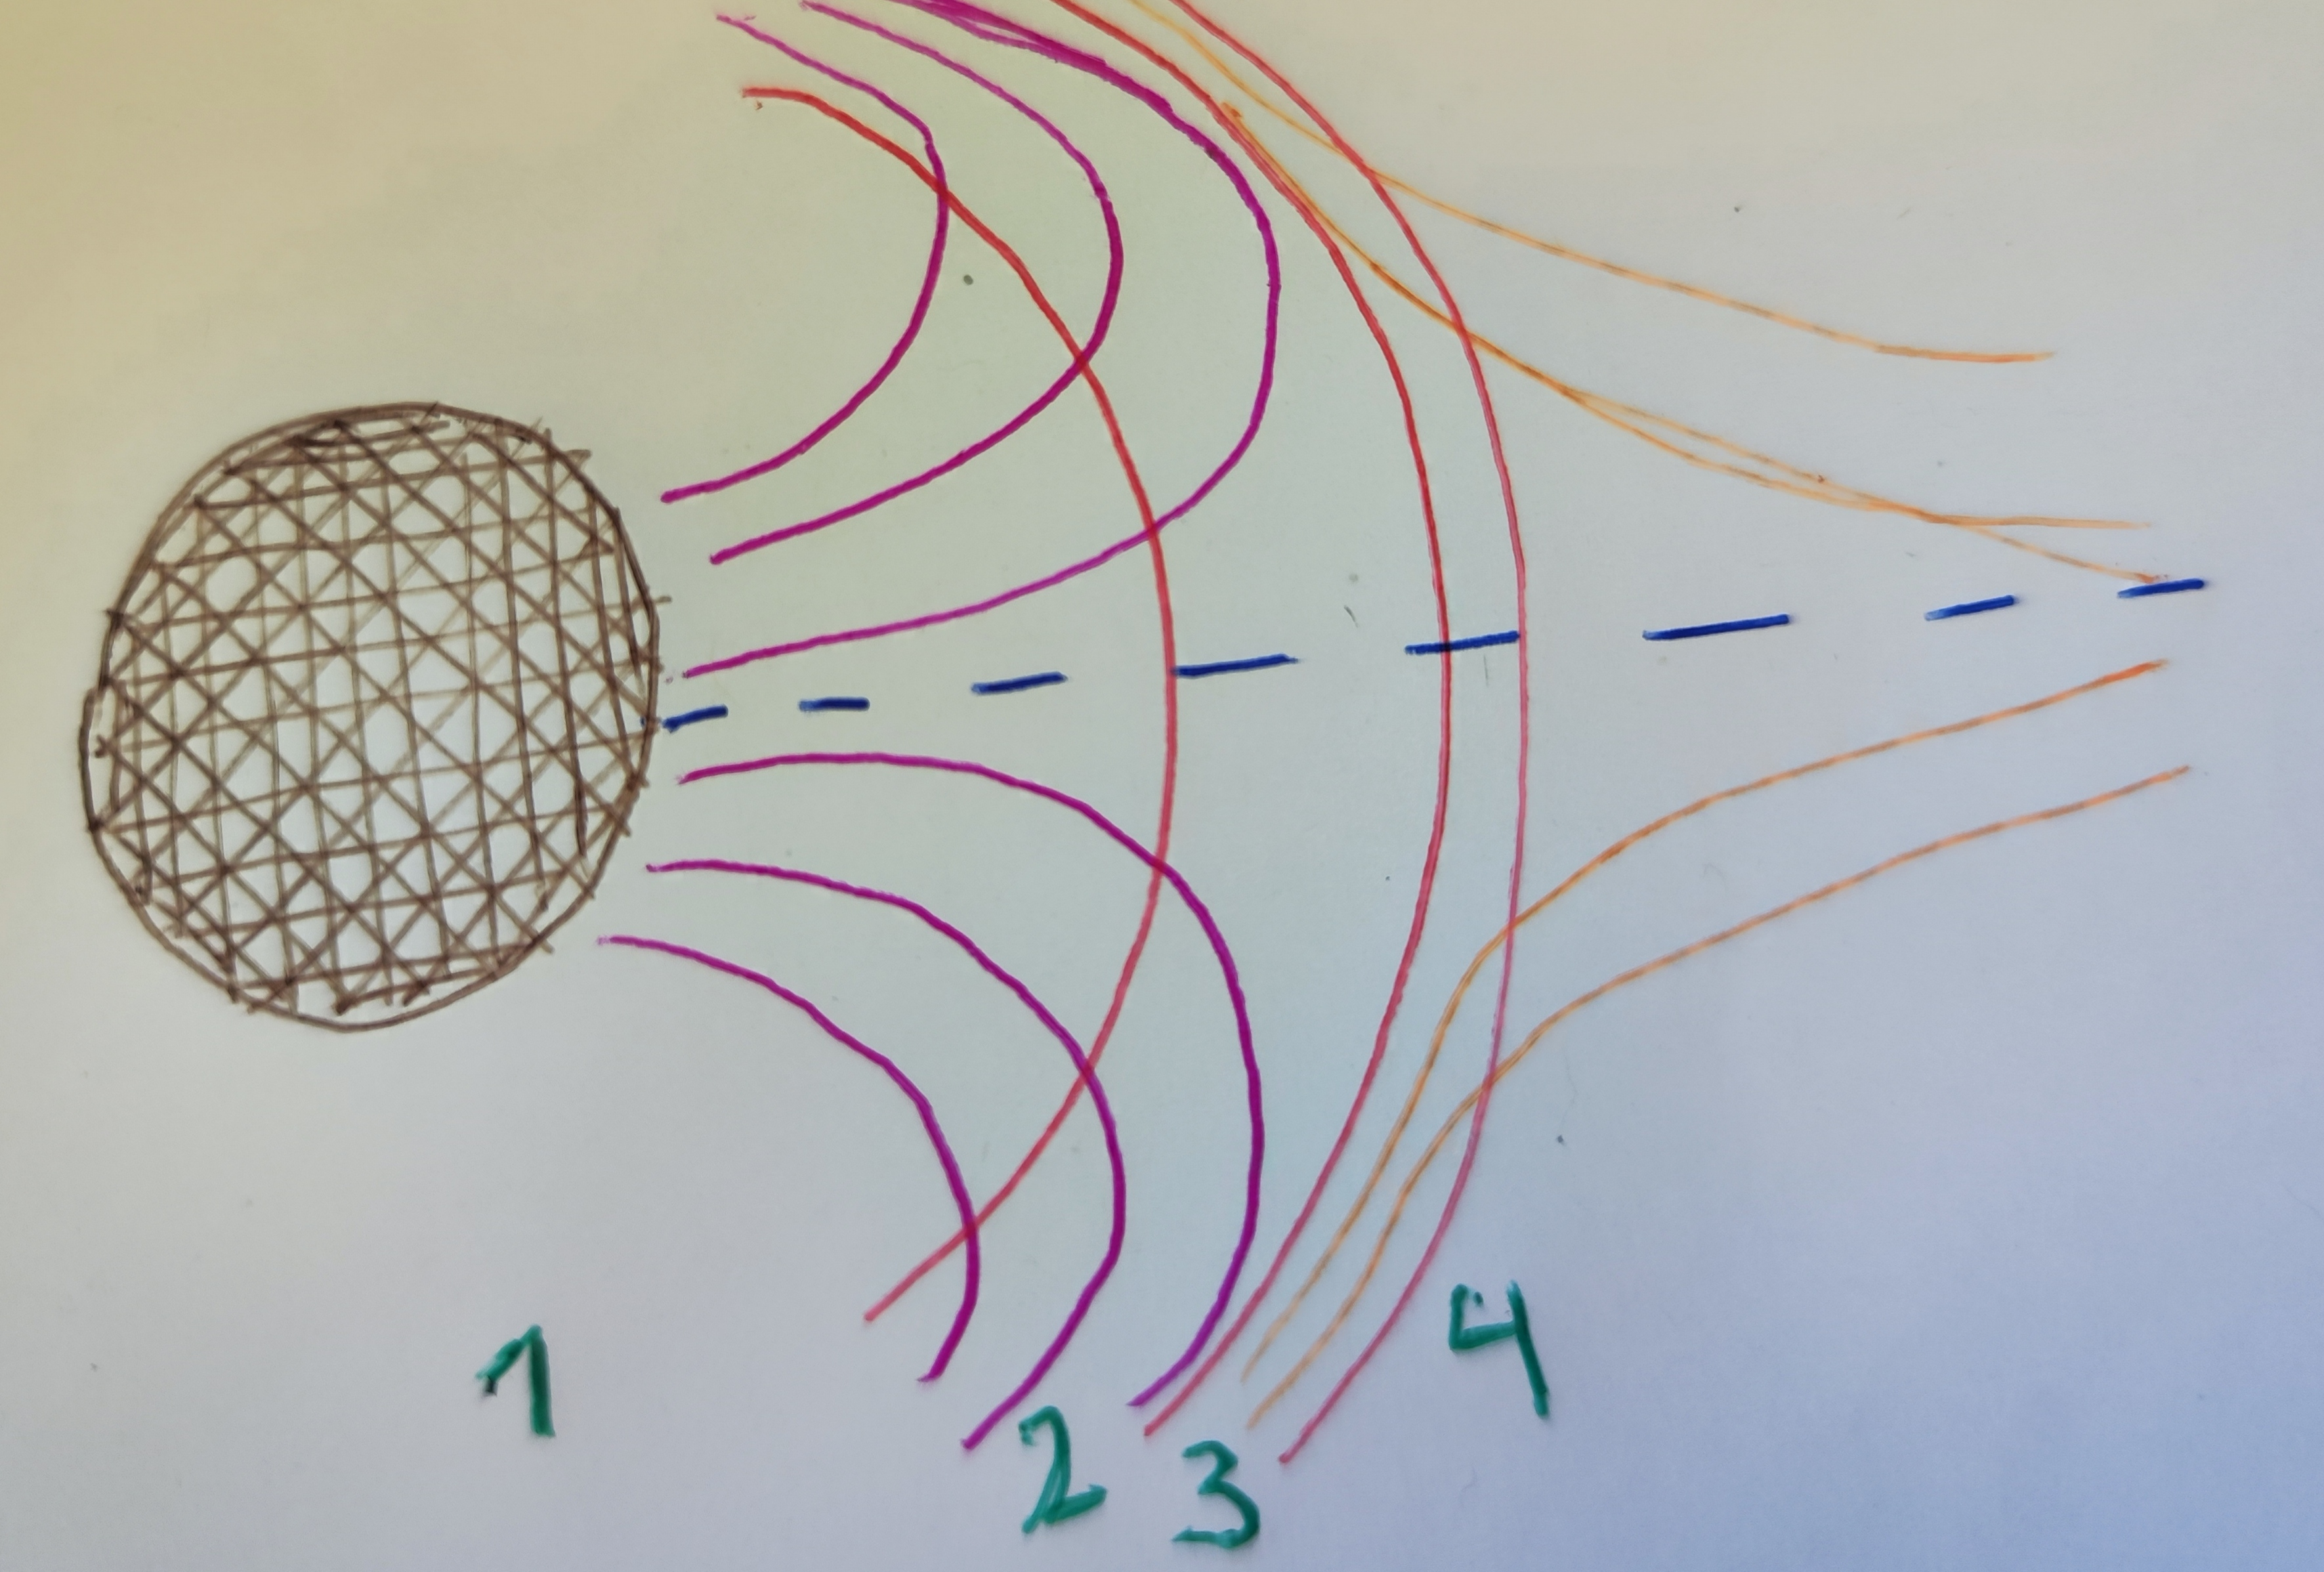
\includegraphics[width=0.75\textwidth]{Chp2_Zone.jpg}
    \caption{E c C.
    Vemos las 4 zonas que se forman en la interacción entre el flujo fotoevaporativo y el viento estelar de una estrella. La línea punteada es el eje de simetría que vamos a considerar para tomar este problema de manera unidimensional. la zona 1 es donde el flujo fotoevaporativo sale de la superficie del glóbulo con un número de Mach 1 y va aumentando, la zona 2 es el flujo fotoevaporativo chocado, la cual esperamos ver en las observaciones como una cáscara,, la zona 3 es el viento chocado y la zona 4 es donde viaja el viento estelar, el cual es menos denso que el flujo fotoevaporativo.}
    \label{fig:zones}
\end{figure}

La interacción entre el flujo fotoevaporativo y el viento estelar puede ser diferente morfológicamente, dependiendo si el flujo fotoevaporativo es isotópico o anisótropo. Por lo que en un principio vamos a tratar este problema de manera radial con una simetría cilíndrica con respecto a un eje de simetría, en la cual consideraremos un ángulo preferencial, de esta manera si ignoramos las variaciones transversales lo trataremos como un problema unidimensional.

\begin{figure}[h]
    \centering
    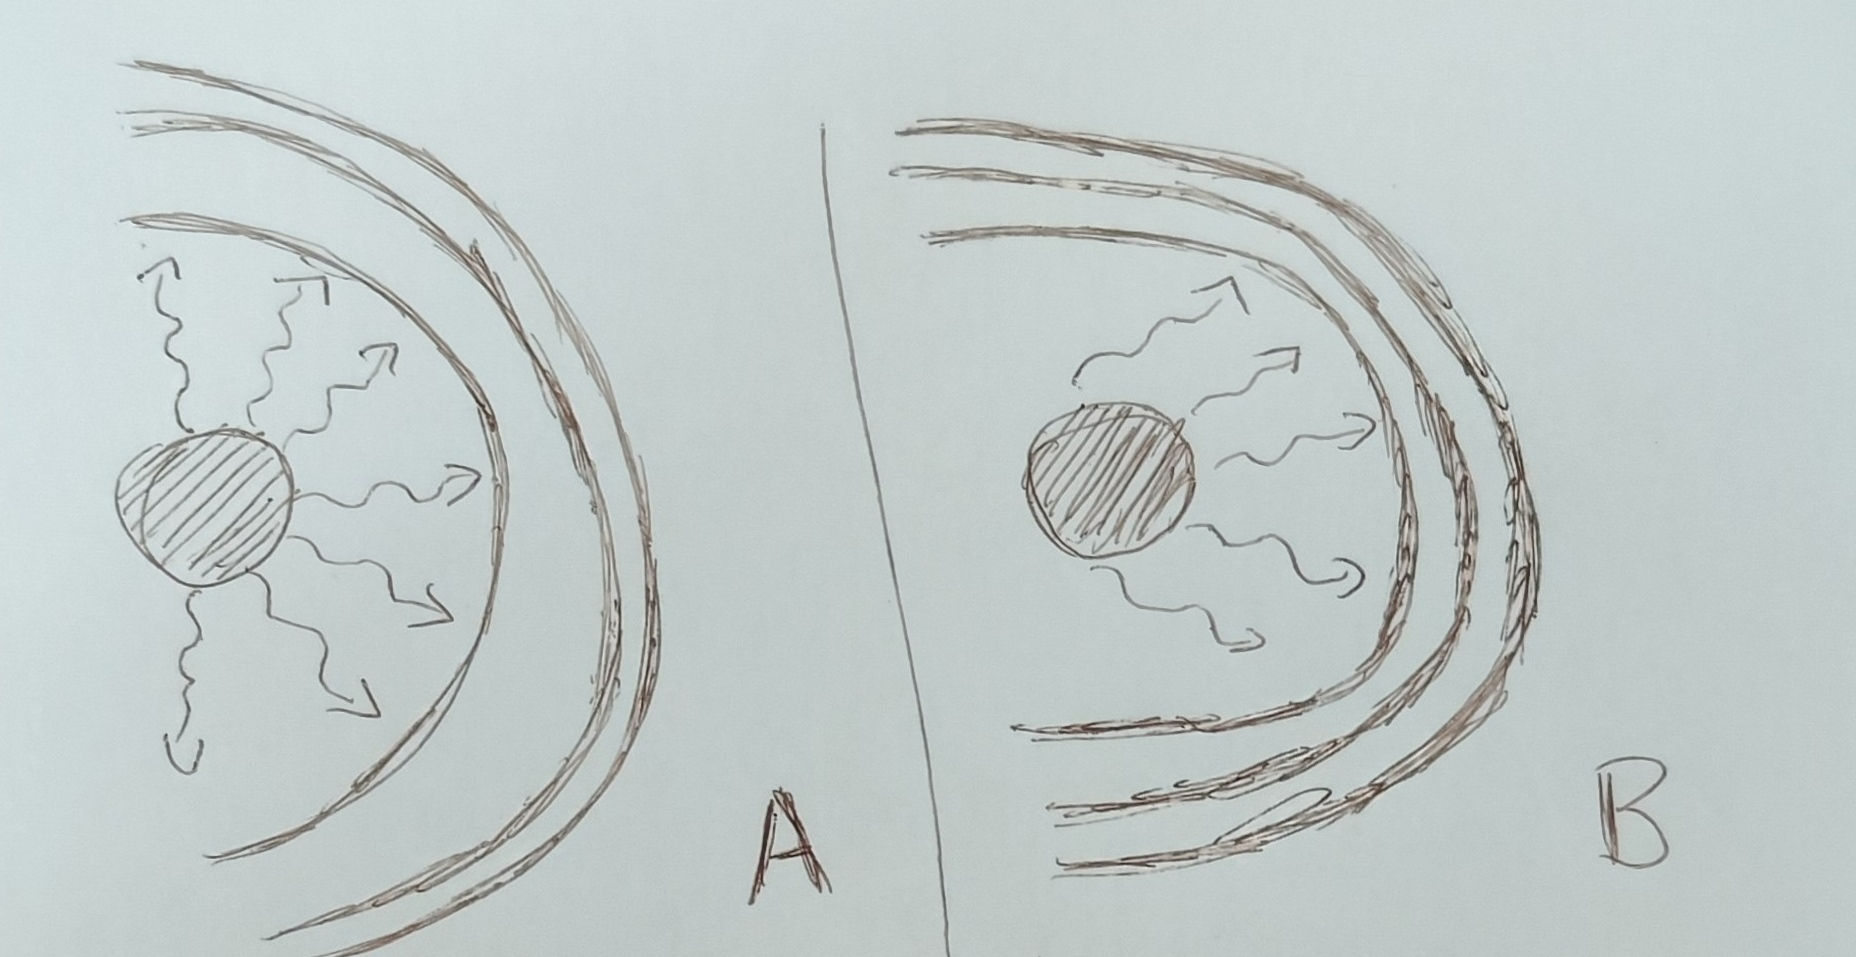
\includegraphics[width=0.75\textwidth]{Chp2_iso&ans.jpg}
    \caption{\textbf{A} es la interacción de un fujo fotoevaporativo isotópico con un viento externo y \textbf{B} es la interacción de un flujo fotoevaporativo anisótropo con un viento externo. Vemos que en el caso isotópico se nos es más fácil tratar las diferentes regiones de manera radial debido a la geometría.}
    \label{fig:isotyaniso}
\end{figure}

Dado que el flujo fotoevaporativo es más denso que el viento estelar, esperamos ver solo el flujo fotoevaporativo chocado y no el viento estelar chocado, ya que esperamos que este sea no radiativo.

\begin{figure}[h]
    \centering
    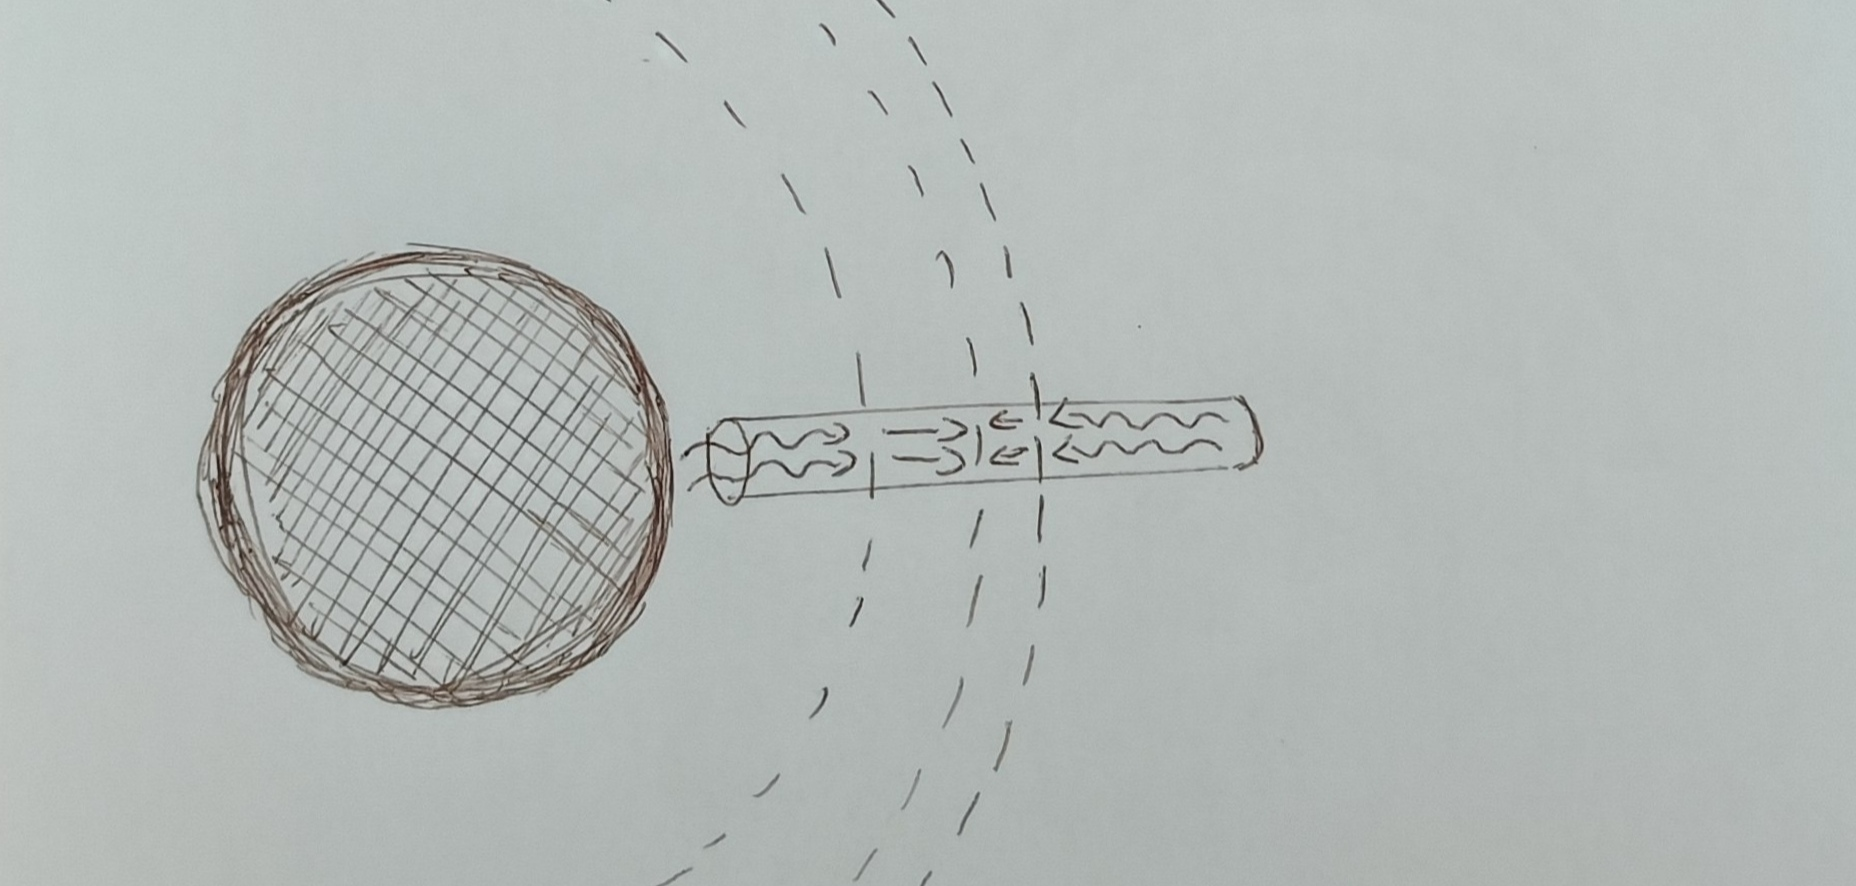
\includegraphics[width=0.75\textwidth]{Chp2_cilinders.jpg}
    \caption{Si consideramos una simetría cilíndrica con un radio muy pequeño, podemos tratar este problema de manera radial y de tal manera que la radiación y el viento estelar inciden de manera perpendicular al glóbulo.}
    \label{fig:cilinders}
\end{figure}

\section{Estimación de la densidad ionizada a partir del brillo superficial de $H_\alpha$}

Para estimar la densidad ionizada, usamos primero la definición de medida de emisión (EM por sus siglas en inglés)
\[EM=\int_z n_in_edz\] donde en este caso estaremos integrando sobre nuestra línea de visión. Esta EM depende tanto de la densidad de electrones como de iones, pero en nuestro caso vamos a considerar un equilibrio de ionización entre el flujo foto evaporativo y el viento estelar, por lo que $n_e=n_i$.

Si suponemos una simetría esférica entre esta interacción del flujo fotoevaporativo y el viento estelar, podemos tomar, por geometría, que
\[EM=2\sqrt{rh}n^2.\]

%Insertar imagen de los radios

Esto ya que de la fig(?) tenemos que por geometría $r^2+\frac{1}{2}l^2=(r+h)^2=r^2+2rh+h^2\approx r^2+2rh\Rightarrow l=2\sqrt{rh}$, por lo que podemos estimar la densidad ionizada a través de la EM como \[n=\sqrt{\frac{EM}{l}}\]

\section{Modelo hidrodinámico estacionario}

Para el caso de nuestro modelo analítico consideraremos un modelo analítico hidrodinámico estacionario, esto ya que consideramos que la interacción entre el flujo foto evaporativo y el viento estelar ha llegado al equilibrio de ionización.

%inseratr imagen de las regiones durante la interaccion
.

Para este modelo consideramos glóbulos relativamente pequeños, de unos 200--300 mili arco segundos de diámetro comparado con su entorno que puede ser unas pocas decenas de arco segundos, además a unos 10--30 arco segundos de la estrella masiva como para que su radiación UV llegue desde un pequeño ángulo e interactúe con el glóbulo, de esta manera podemos decir que la radiación incide perpendicularmente, con respecto al eje de simetría, a la superficie del glóbulo.

En nuestro caso tomamos una simetría cilíndrica en la cual podamos tomar un radio perpendicular de un tamaño muy pequeño como para tomar este problema solo de manera radial, pero notemos que debido a la forma de estos glóbulos, en realidad tendremos una familia de cilindros a cada ángulo, por lo que tomando el radio perpendicular a la radiación muy pequeño, entonces podemos considerar este problema solo de manera radial, un problema unidimensional, en la dirección en la que incide la radiación de la estrella.

En general en el medio interestelar hay muchas fuerzas que afectan el cambio en la materia, pero en este caso vamos a despreciar la fuerza de gravedad, tanto del mismo glóbulo como la gravedad impuesta por la estrella, tampoco vamos a considerar fuerza por campos magnéticos por simplicidad. Por lo que solo vamos a considerar las fuerzas dada por el gradiente de presión por parte del flujo fotoevaporativo, donde tomaremos el viento estelar como condición de frontera.

Para el flujo fotoevaporativo por parte del glóbulo vamos a considerar las ecuaciones de hidrodinámica, la ecuación de conservación de masa ya que como dijimos antes, el tiempo en el que un bulto sale de esta interacción le toma bastante tiempo. Usaremos también la ecuación de Bernoulli para un gas isotermo, donde la velocidad del sonido en este gas dependerá de la temperatura.

% Balance between ionizations and recombinations

\section{Ecuación de estado y equilibrio de ionización}

Para nuestro flujo tomaremos dos presiones, la hidrodinámica y la térmica, por lo que tenemos una presión total dada por
\[P_{tot}=P_{ter}+P_{hid}=n\bar{m}c_s^2+n\bar{m}u^2=\rho c_s^2(1+M^2)\]

En nuestro modelo consideramos que nuestro flujo que sale de la base del glóbulo tiene como condiciones iniciales
\[M=1\]
\[r=r_0\]
\[\rho=\rho_0\]
\[P_{tot}=P_0\]
y en nuestro modelo queremos ver cuando la presión del flujo llega a un equilibrio con la presión RAM del viento estelar, por lo que queremos conocer a que distancia se da, $r_1$, y que densidad y número de Mach tendría, para esto vamos a tomar que la presión disminuyó una fracción de la presión inicial. Por lo que la presión cambia como 
\[\frac{P}{P_0}=\frac{\rho c_s^2(1+M^2)}{\rho_0 c_s^2(1+1)}=\frac{\rho}{\rho_0}\frac{1+M^2}{2}\]
Considerando la ecuación para la conservación de masa tenemos que
\[\rho r^2M	=\rho_0 r_0^2\]
y finalmente si consideramos la ecuación de Bernoulli isotérmica 
\[\dots\]
de la cual tenemos 
\[\frac{r}{r_0}=M^{-1/2}e^{\frac{M^2-1}{4}}\]
Ahora que tenemos tres ecuaciones y tres incógnitas podemos resolver, en nuestro caso lo hicimos de manera numérica. Al resolver estas ecuaciones para diferentes $f$ tenemos que tanto la presión como la densidad decaen con el radio, mientras que el número de Mach aumenta.

%Imagen temporal de como depende la densida, presio y M como funcion del radio 



% Assumption of isothermal equation of state

% General solution for the internal structure of model


\chapter{Aplicación a M1-67}

\section{Observaciones con HST}

\section{Observaciones con JWST}

\section{Ajustando el modelo a los perfiles de brillo radial}

\section{Estimando la presión RAM del viento estelar}

\section{Estimando la tasa de foto ionización}

\chapter{Conclusiones}

\appendix
\chapter{Estimación de fuerzas en el modelo}

\bibliography{references}

\end{document}
